\documentclass{article}
\usepackage{graphicx}
\title{Gwent - Pro Informe}
\author{Darian Santamarina Hernandez}
\date{\today}

\begin{document}

\maketitle
En este informe se presenta el Primer Proyecto de Programación de Primer Año Curso 2024
\centering
\setcounter{secnumdepth}{0}
\section{Estructura del Informe}
-Diseño de las Cartas\\
-Cartas\\
-Deck\\
-Robar\\
-Invocar
-Efecto\\
-Sistema de Turnos\\
-Sistema de Rondas\\
\begin{figure}
\centering
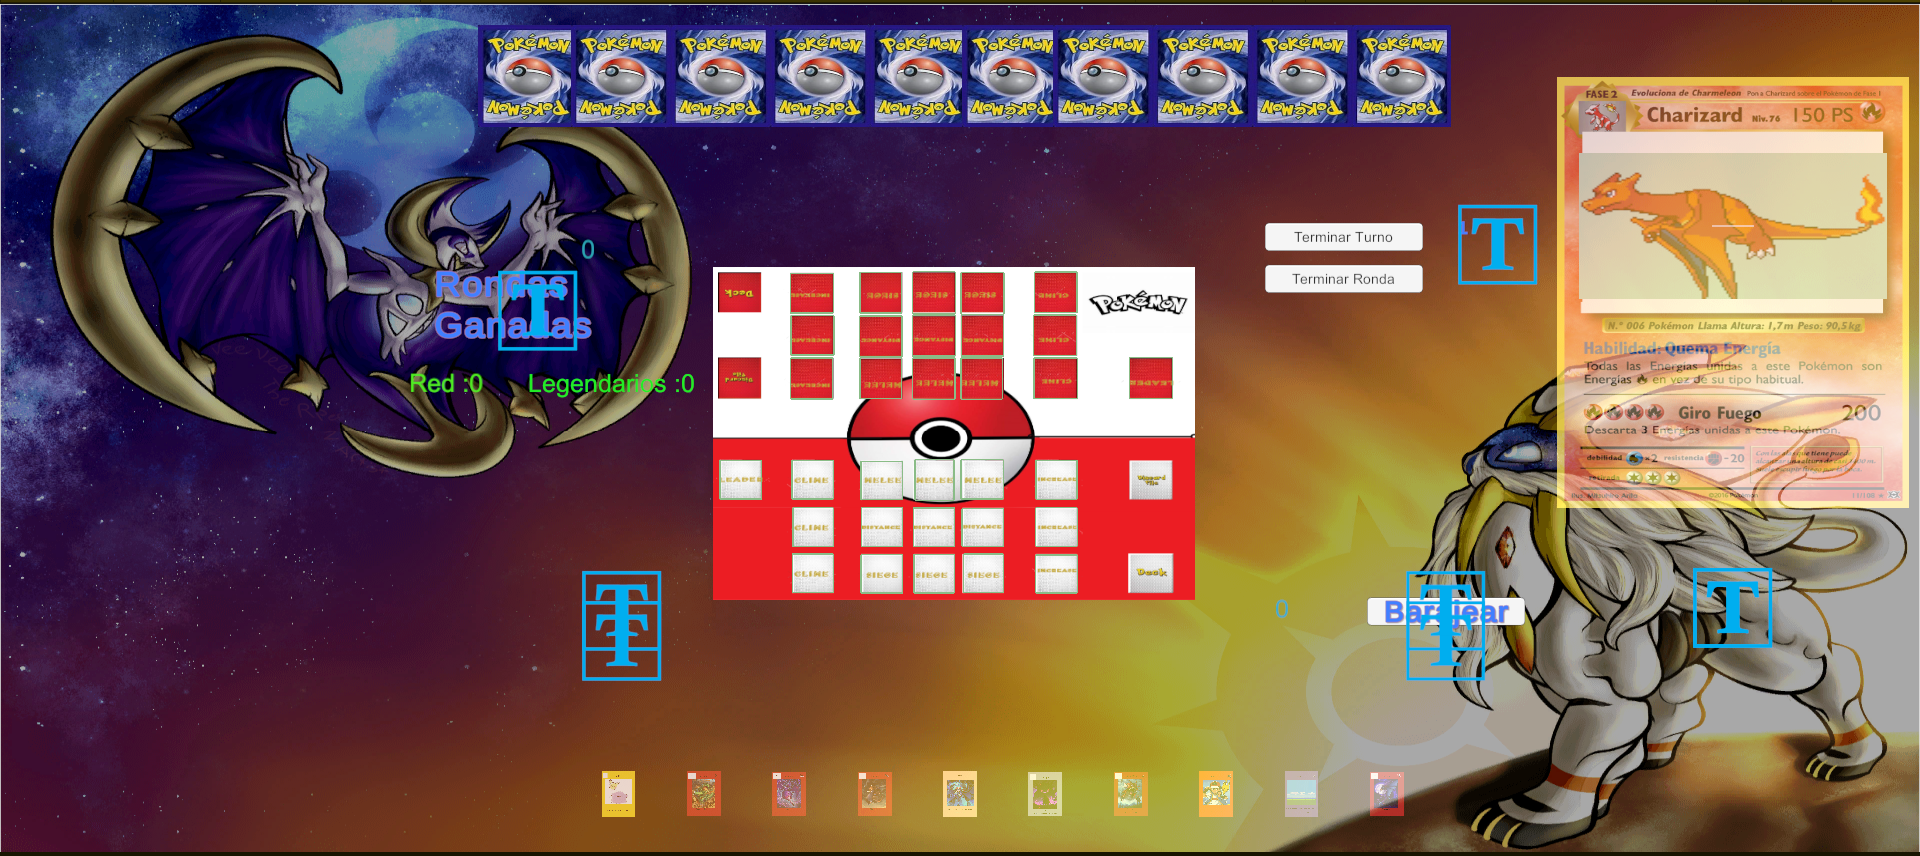
\includegraphics[width =1\textwidth]
{1}
\caption{Escena del juego principal}
\label{fig : a}
\end{figure}
\newpage
\centering
\setcounter{secnumdepth}{0}
\section{Diseño de las Cartas}
Al diseñar cartas, ya sea para juegos, tarot, cartas coleccionables o cualquier otro propósito, es crucial considerar la estética, la legibilidad y la coherencia visual para garantizar una experiencia atractiva y funcional para los usuarios. En este contexto, el uso de herramientas especializadas como Nandeck puede jugar un papel fundamental en la creación de cartas bien diseñadas y visualmente atractivas.(Esto seria mis Sprites de cada Carta)
\subsection{¿Que es Nandeck?}
Nandeck es una herramienta de creacion de cartas, atraves de la programacion y automatizacion de las mismas con una interfaz facil de trabajar , y una libertad fascinante para crear diseños completamentes unicos.
\begin{figure}
\centering
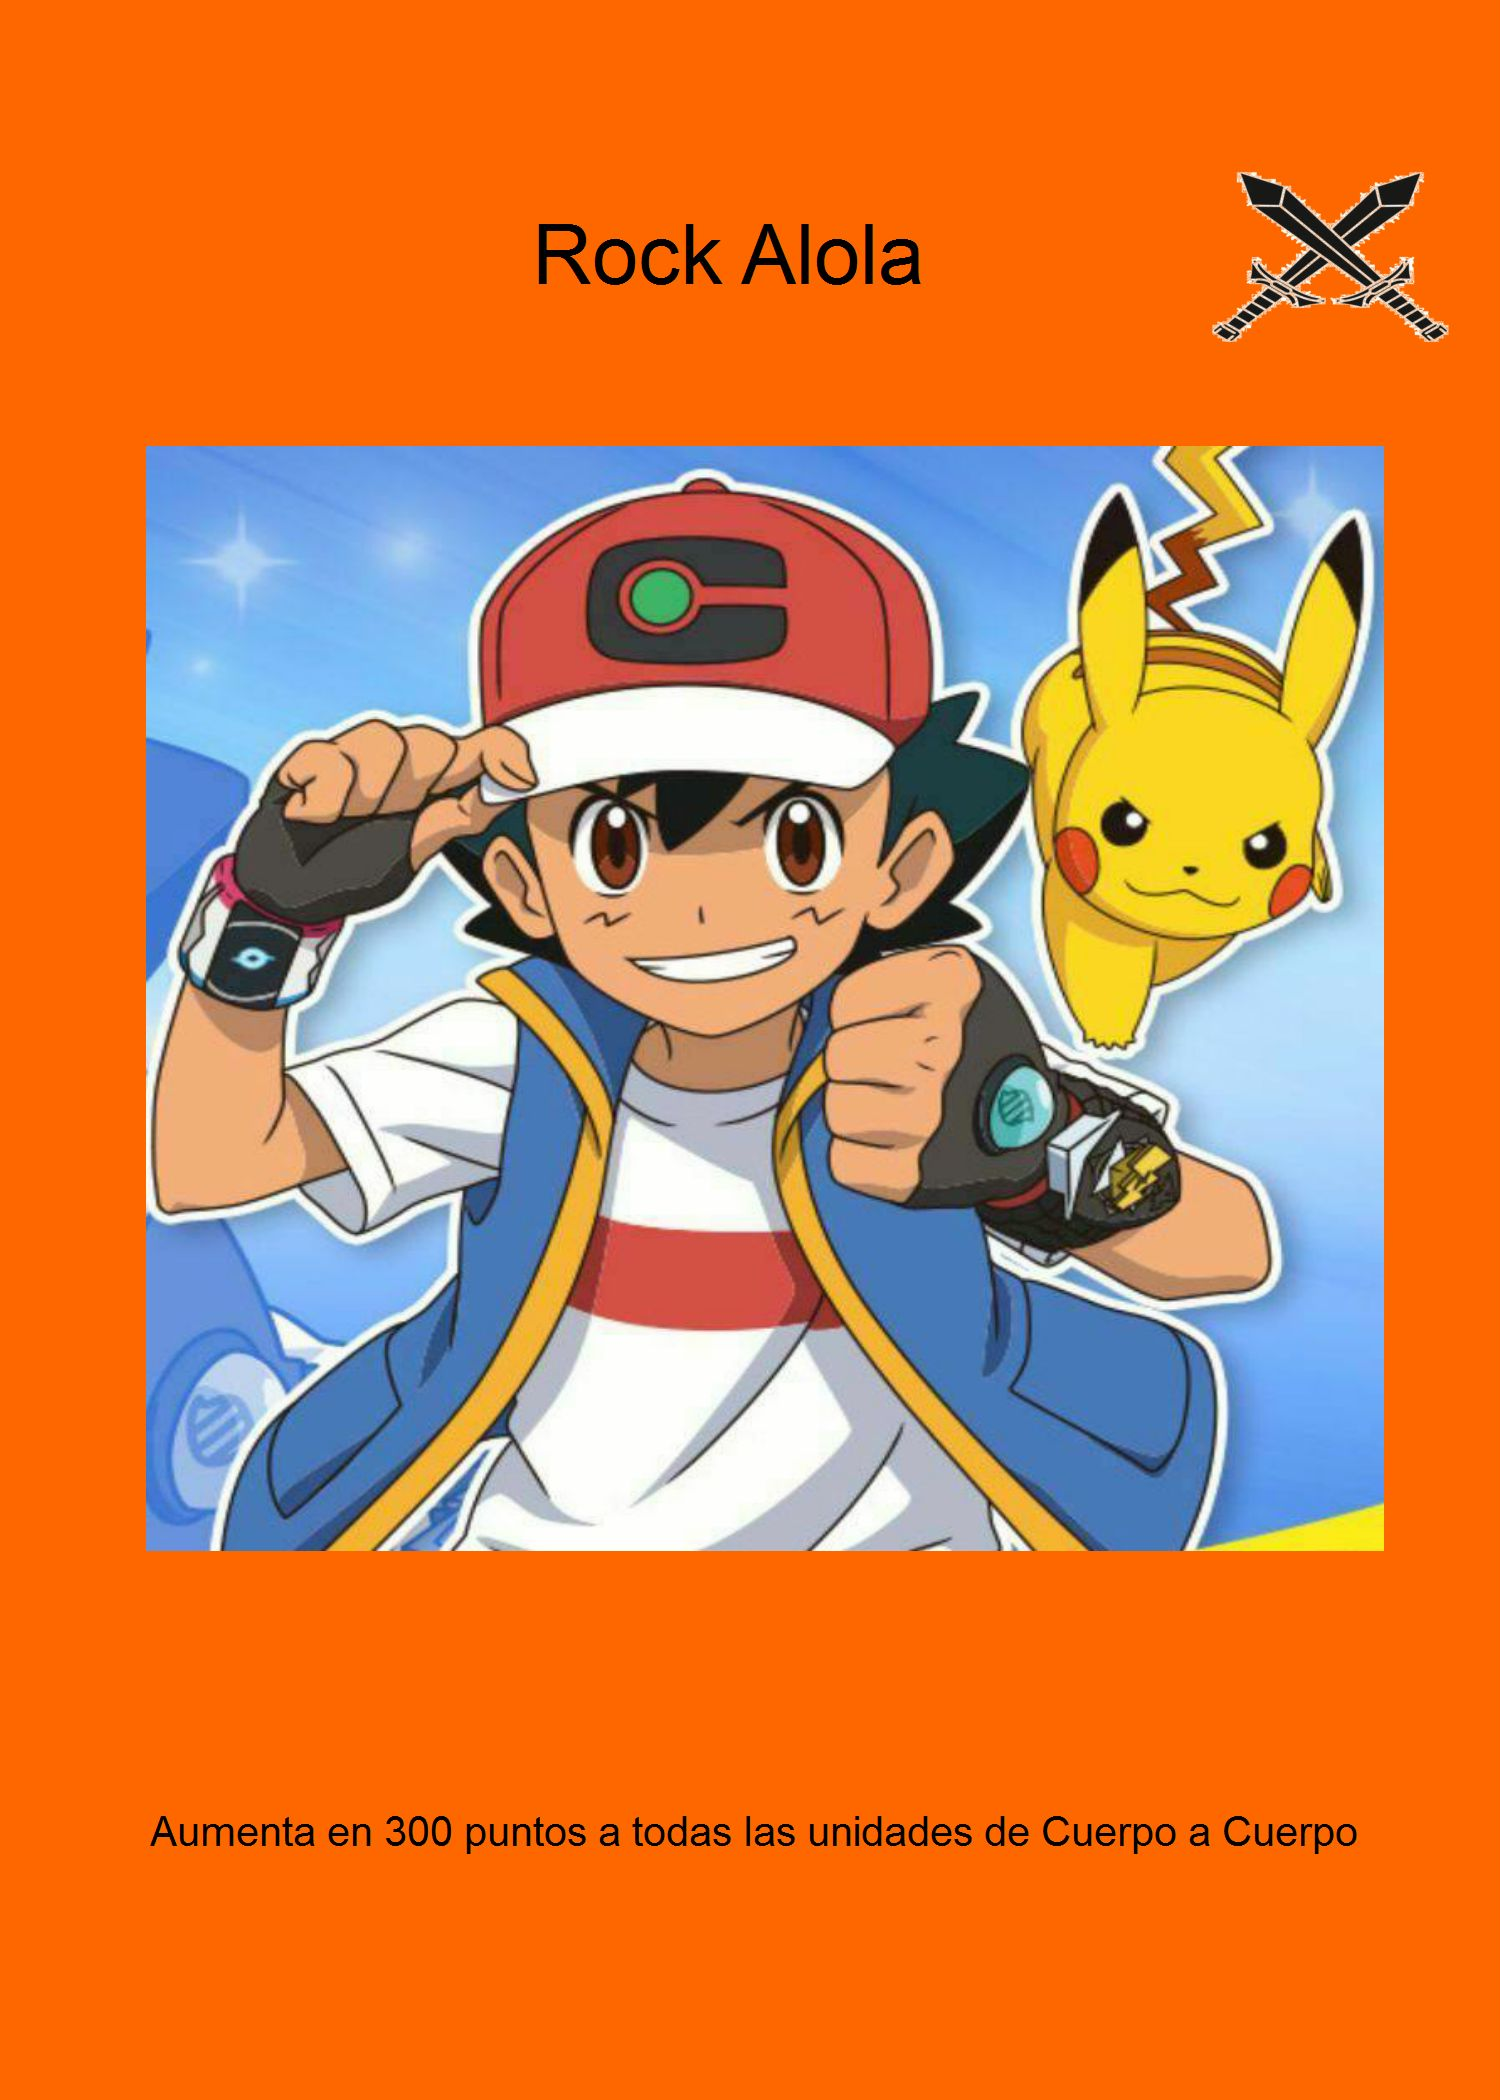
\includegraphics[width =1\textwidth]
{Aumento3}
\caption{Ejemplo de un Sprite disenado en NandDeck}
\label{fig : a}
\end{figure}
\newpage
\subsection{Cartas}
Las cartas en el juego se representan a traves de prefabs de Gameobjects ,adjunto a cada prefab de GameObjcets viene un Script llamado CardUnidad , q le dara propiedades a las cartas  , ataque , tipo , nombre y efecto .Los Sprites de cada carta , osea la imagen fisica, tmb estara adjunto a cada prefab y fue colocada una por una a cada Carta correspondiente.
\section{Deck}
Cuando se tiene cada carta como un prefab , estas seran colocadas dentros de un GameObject el cual tendra adjumto , otros script llamado Deck , el cual se encargara de tener una lista , el cual tendra 25 cartas pertencientes a un solo bando del juego , asi mismo para el deck rival. 
\begin{figure}
\centering
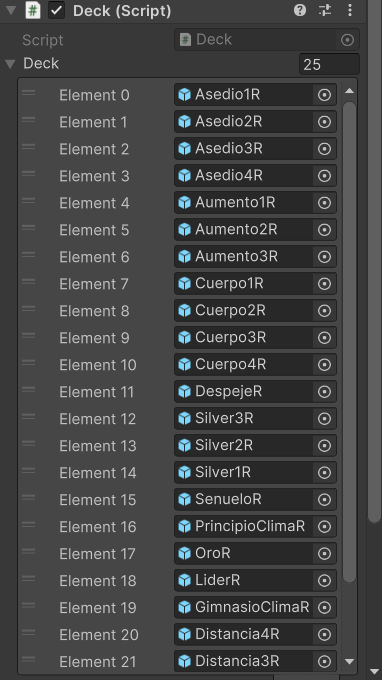
\includegraphics[width =0.5\textwidth]
{5}
\caption{Ejemplo de un deck}
\label{fig : a}
\end{figure}
\newpage
\section{Robar}
Aqui es una funcion bastante sencilla , al iniciar el juego se selecciona aletoriamente , de mi deck (osea los prefabs de mis cartas) , 10 numeros al azar q sera la 10 cartas del inicio del juego , asi mismo para el rival.
\subsection{Posiciones de las Cartas}
Dentro de cada deck existiran  un objecto vacio q representara ambas manos,cada una de estas manos contara a la vez con objectos vacios q tendran ambos una posicion especifica dentro de mi canvas , osea tendria 10 espacios vacios en cada lado del canvas(campo) , entonces mi funcion lo q hara es buscar los gameobjects ubicados en las posiciones vacias y despues de Instaciado cada uno de mis prefabs sacados aleatoriamente, le cambiara la posicion a cada uno y las colocara encima de mis posiciones vacias.
\subsection{Barajear}
La opcion de Barajear es un boton q se agraga, para en el principio del juego , ambos jugadores tiene la posiblidad de devolver dos cartas de su mazo a su mano , esta funcion trata de primeramente remover todas las inntancias de las cartas sobre el campo y destruirlas , a la par removemos 2 cartas de la mano , las colacamos en el deck , y anadimos dos prefabs mas a la mano y instanciamos y hacemos el mismo proceso q al principio del juego para colocar las 10 cartas en sus posiciones correspondientes.
\begin{figure}
\centering
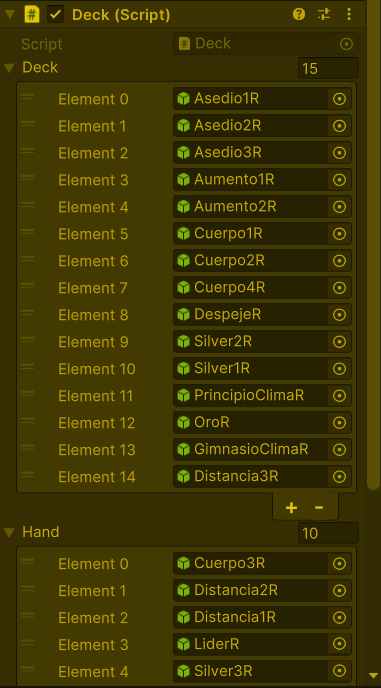
\includegraphics[width =0.5\textwidth]
{2}
\caption{Lo q le sucede a un deck cuando inicia el juego , osea se roban las cartas}
\label{fig : a}
\end{figure}
\newpage
\section{Invocar}
La funcion de Invocar en mi programa es posiblemente la funcion mas compleja de todas , este Script va adjunto a los prefabs de las cartas igual ,tengo preparado en el campo de batalla osea el tablero , objectos vacios para los cuales tener una referencia a la posicion a la q quiero poner las cartas invocadas , ademas coloque en cada prefab colliders para hacer interactuables mis objectos en el canvas, con la funcion OnMouseDown de Unity hago q para cuando el jugador toque encima de una carta se despligue un panel , q tendra tres opciones(Botones):\\
-Invocar\\
-Efecto\\
-Regresar.\\
Entonces en la funcion de esta seccion (Invocar),ya tenemos las condiciones necesarias para realizarla,al entrar en la funcion hacemos hijo del Canvas a toda carta q sea invocada en el juego, y tendriamos q comprobar dos cosas q las posicion sea del mismo tipo q la carta (lo verifico por Tag) , y q la posicion ya no ha sido previamente ocupada por otra carta (este proceso lo hago a traves de una mascara boolena, donde tengo abstractamente un tablero con las cartas ocupadas en true o false segun si ha sido ocupadas o no) y mi invocacion viene siendo tomar las coordenas de la posicion vacia en el campo y darle esa misma coordena al objecto instanciada de mi mano.
\begin{figure}
\centering
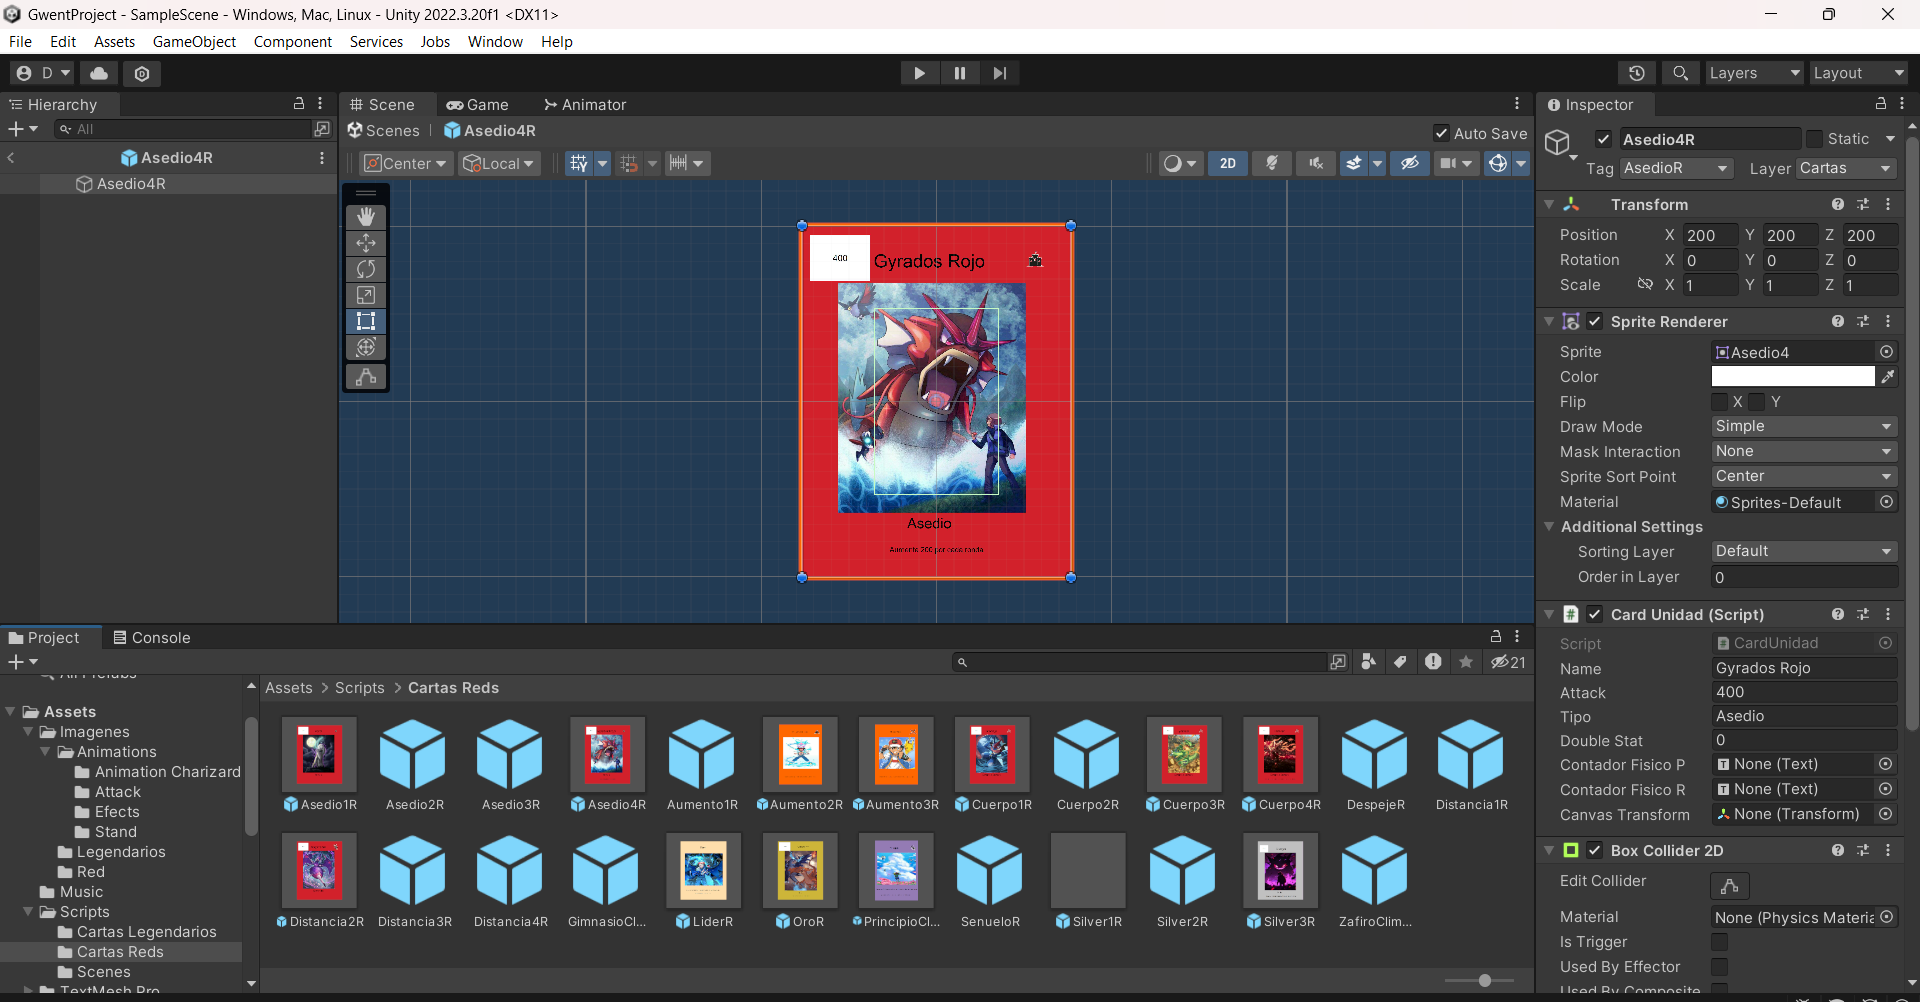
\includegraphics[width =1\textwidth]
{4}
\caption{Representacion de las propiedades de una carta}
\label{fig : a}
\end{figure}
\newpage
\section{Efecto}
Efecto es otra opcion q tiene el jugador al tocar una carta , la funcion trata de ver si la carta jugada tiene un efecto o no , si lo tiene tendra una mascara boleana q comprobora q el efecto no se active mas de una vez , los efectos en el juego son muy variadas , lo mas comunes son la suma y resta de puntos por filas en las cartas aumento o de clima(basicamente me aprovecho de q hay una mascara booleana creada para las cartas invocadas y depedendiendo en q fila esta aplicado calculo la cantidad de true q hay y lo multiplico por la cantidad q diga la carta), otro efecto curioso seria despeje q seria eliminar una carta clima sobre el campo , basicamente lo q hago es encontrar q carta tipo clima tengo en el canvas y la envio al cementerio(mi cementerio es una coordena muy lejos de la escena).
\newpage
\section{Sistemas de Turnos}
En el script BottonSettings fue creado con el objectivo de tener dos botones , uno para el cambio de Turno y otro para el cambio de Ronda,
Para cambiar de turno , como es un juego q se juega en la mismsa pantalla , la Main camara de Unity , osea su camara principal se gira 180 grados para dar un efecto de cambio de turno , q las cartas del rival se muestren correctamente , tanto como Ronda como Turnos ambos tendran un contador Text Mesh Pro , el cual se encargara de reflejar en pantalla el numero de Turnos jugados y Rondas.
\section{Sistema de Rondas}
Los Rondas son un poco mas complejas ,se trata de declarar un ganador al final de cada una , quien gane dos rondas , gana el juego.\\ 
¿Como se determina el ganador?
En la escena del juego contara con dos Contadores de Puntos , lo cual seran dos objectos tipo Text , pero seran dos numeros , los cuales se comparan al final de cada Ronda y el jugador con mas poder de ataque es el q gana la ronda.\\
¿Cuales son las condiciones para terminar una ronda?
El jugador q comenzo de ultimo es el q decide , despues de pasado 6 turnos cuando se termina la ronda.\\
Al principio de cada Ronda nueva , a traves del Sistema de la rotacion de la camara q se describio anteriormente , empieza la ronda siguiente el ganador de la ronda.Y despues se vacia el campo , osea todas las intancias de las cartas invocadas se trasladas hacia el cementerio , puedo obtener sencillamente cuales cartas ha sido invocadas ya q es simplemente buscarlas en el canvas a la q pertenecen (osea son hijos).
\newpage
\section{Detalles Visuales}
\subsection{Tablero}
El tablero fue disenado con una Aplicacion Online llamada Canvas
\subsection*{Menu}
El menu fue disenado en el canvas y con el cambio entre Escenas es q se conecta con el juego principal , la imagen de fondo q se ve es un panel , y los botones fueron hecho a traves Text Mesh Pro , pero lo mas interesante es el movimiento q tiene al arrastrar el raton , lo cual le da un toque mas vivo al menu interectactuable.
\begin{figure}
\centering
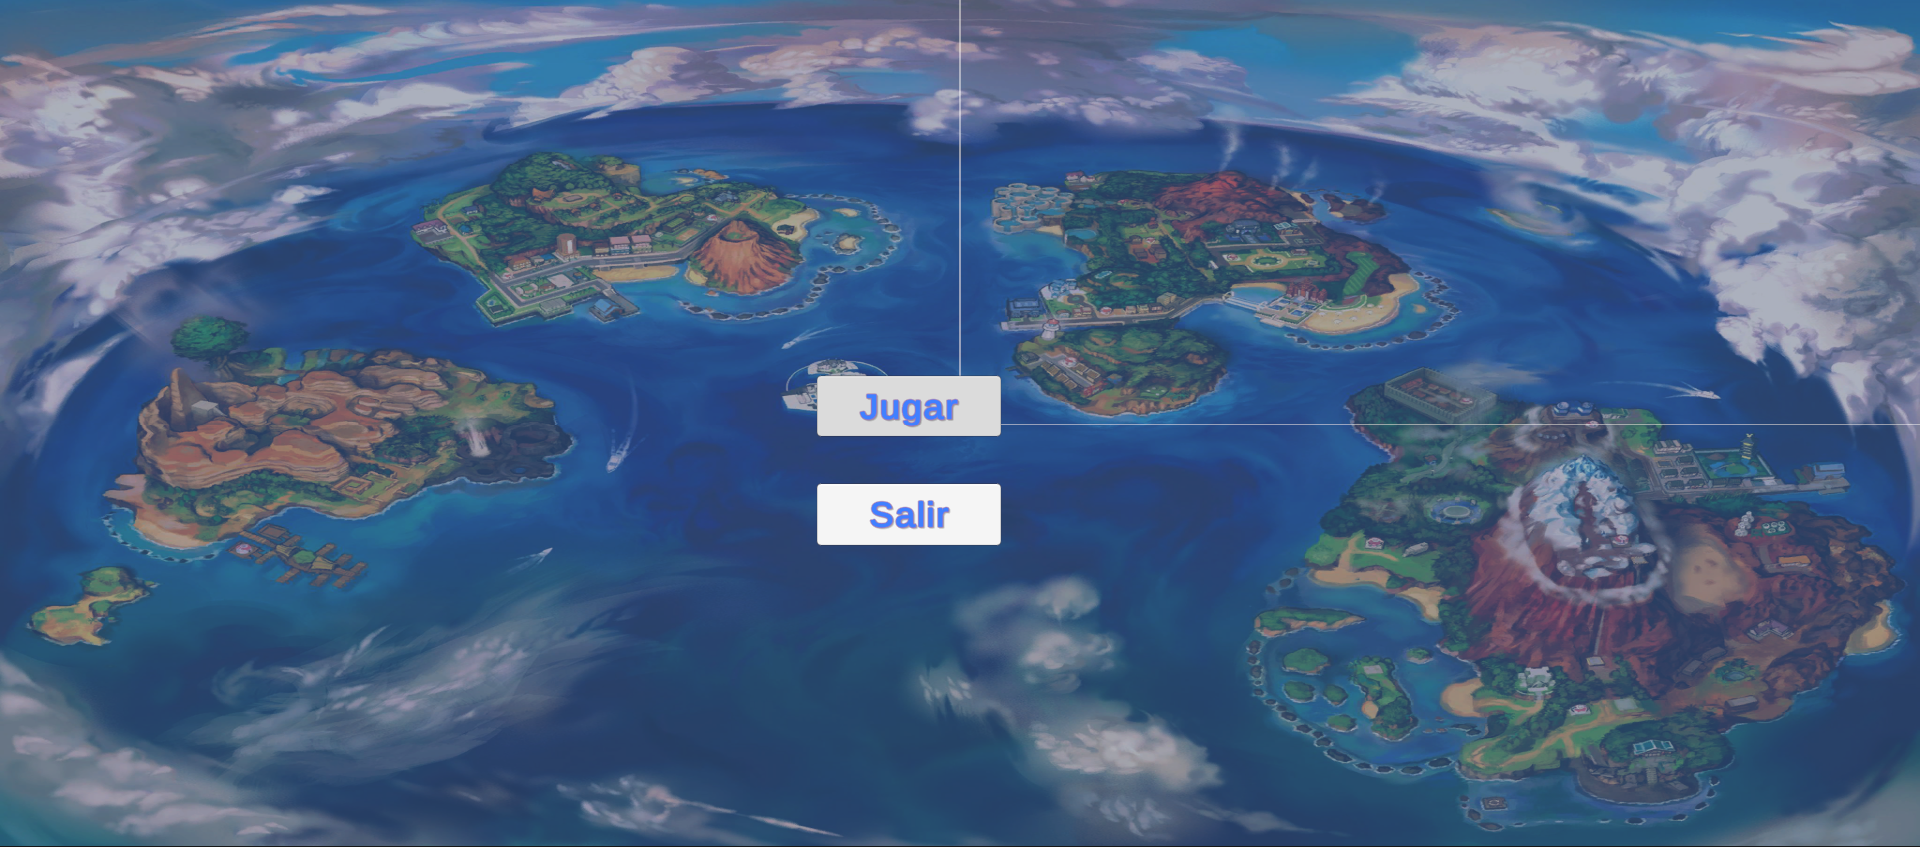
\includegraphics[width =0.5\textwidth]
{3}
\caption{Menu del juego}
\label{fig : a}
\end{figure}
\end{document}